
%%%%%%%%%%%%%%%%%%%%%%%%%
%%%
%%%%%%%%%%%%%%%%%%%%%%%%%
\begin{frame}\frametitle{Combination of \wbx\ and \htx}
\centering\footnotesize

\begin{minipage}{.5\textwidth}\centering
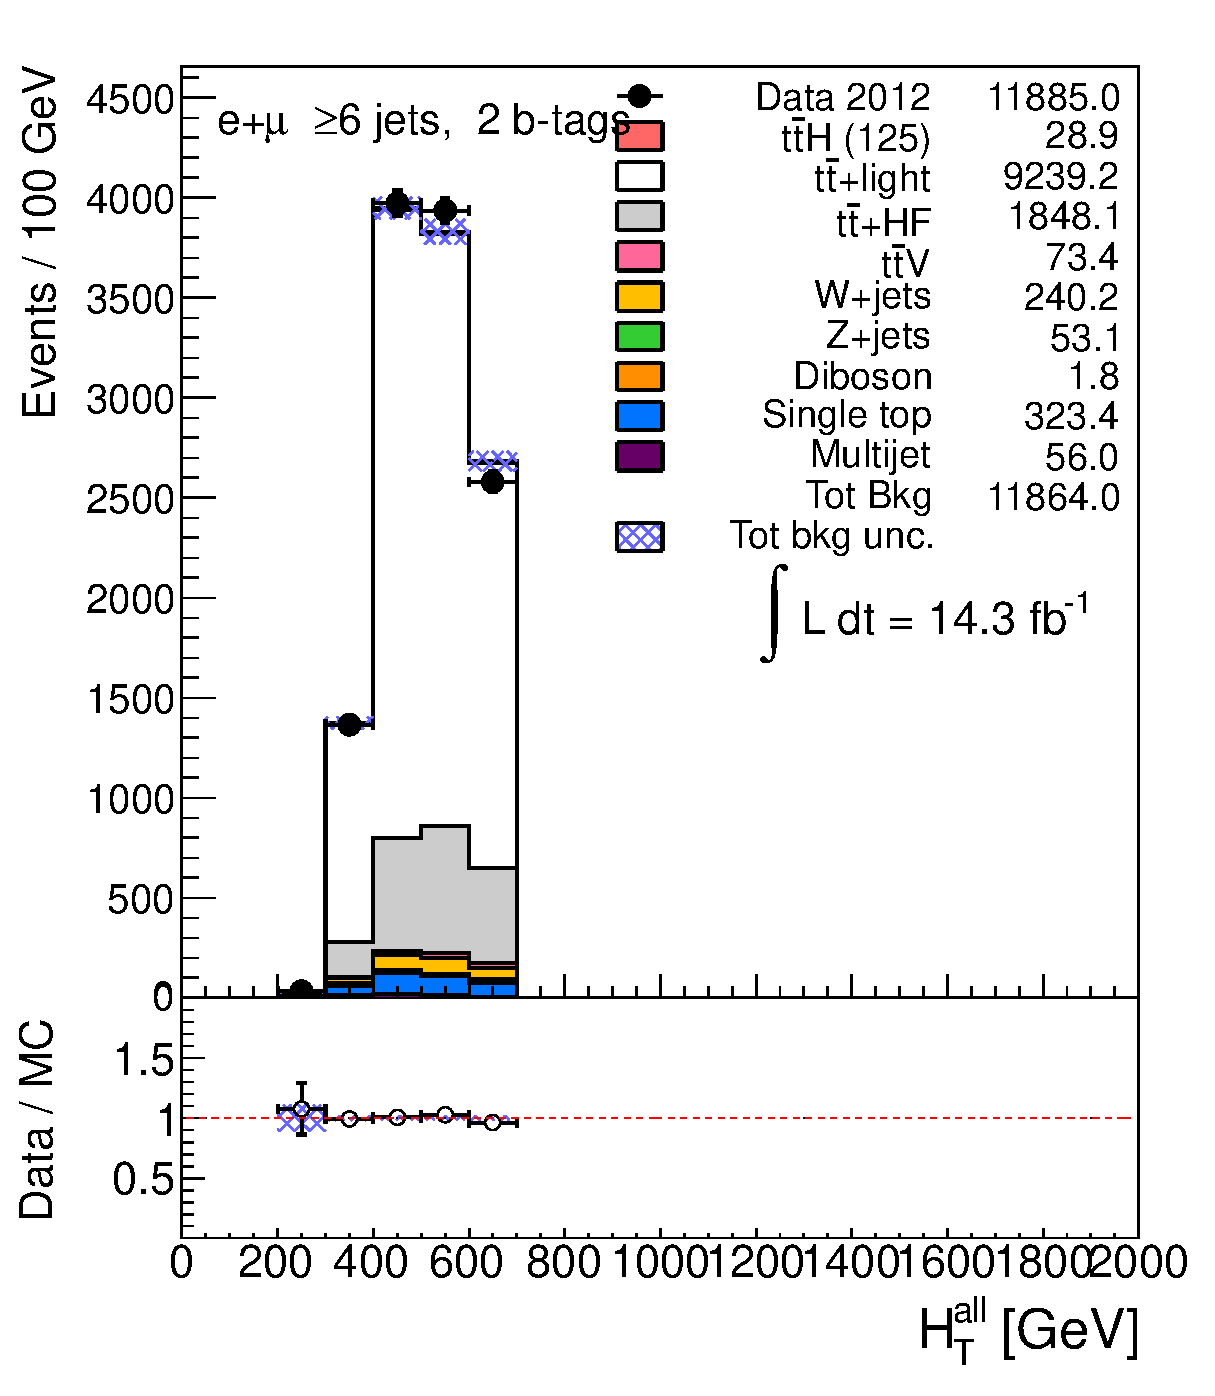
\includegraphics[width=.5\textwidth]{pics/combo/HTAll_6jetin2btagex_ELEMUON}
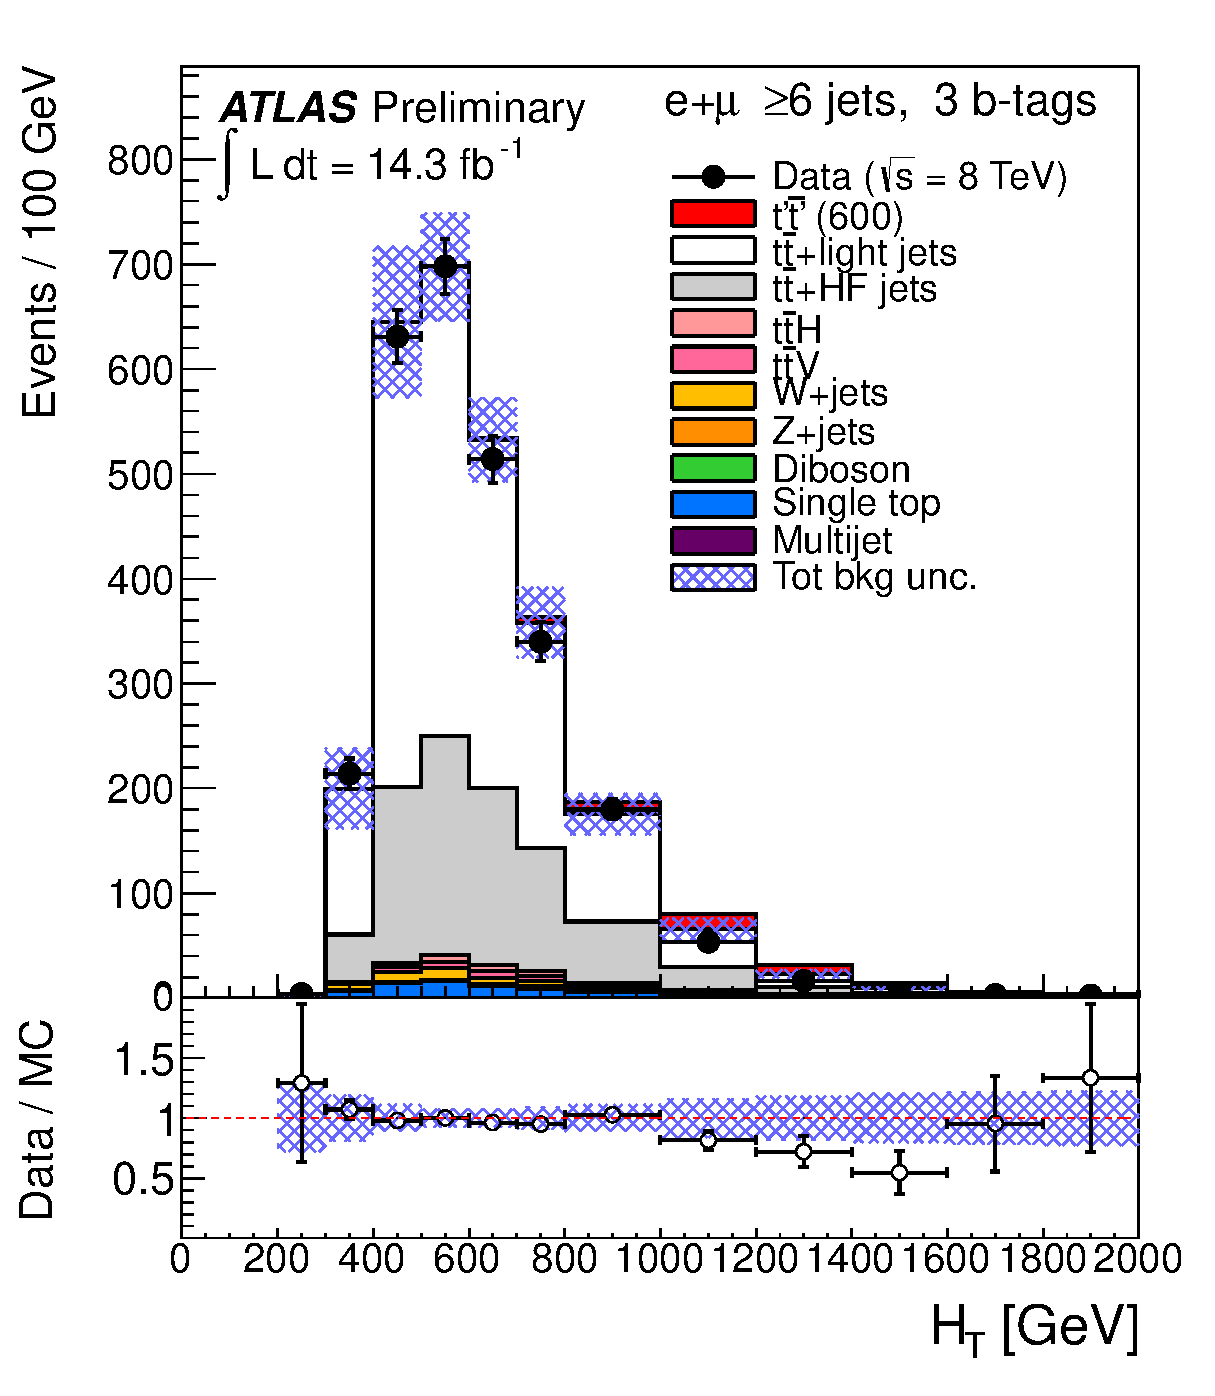
\includegraphics[width=.5\textwidth]{pics/combo/HTAll_6jetin3btagex_ELEMUON}\\
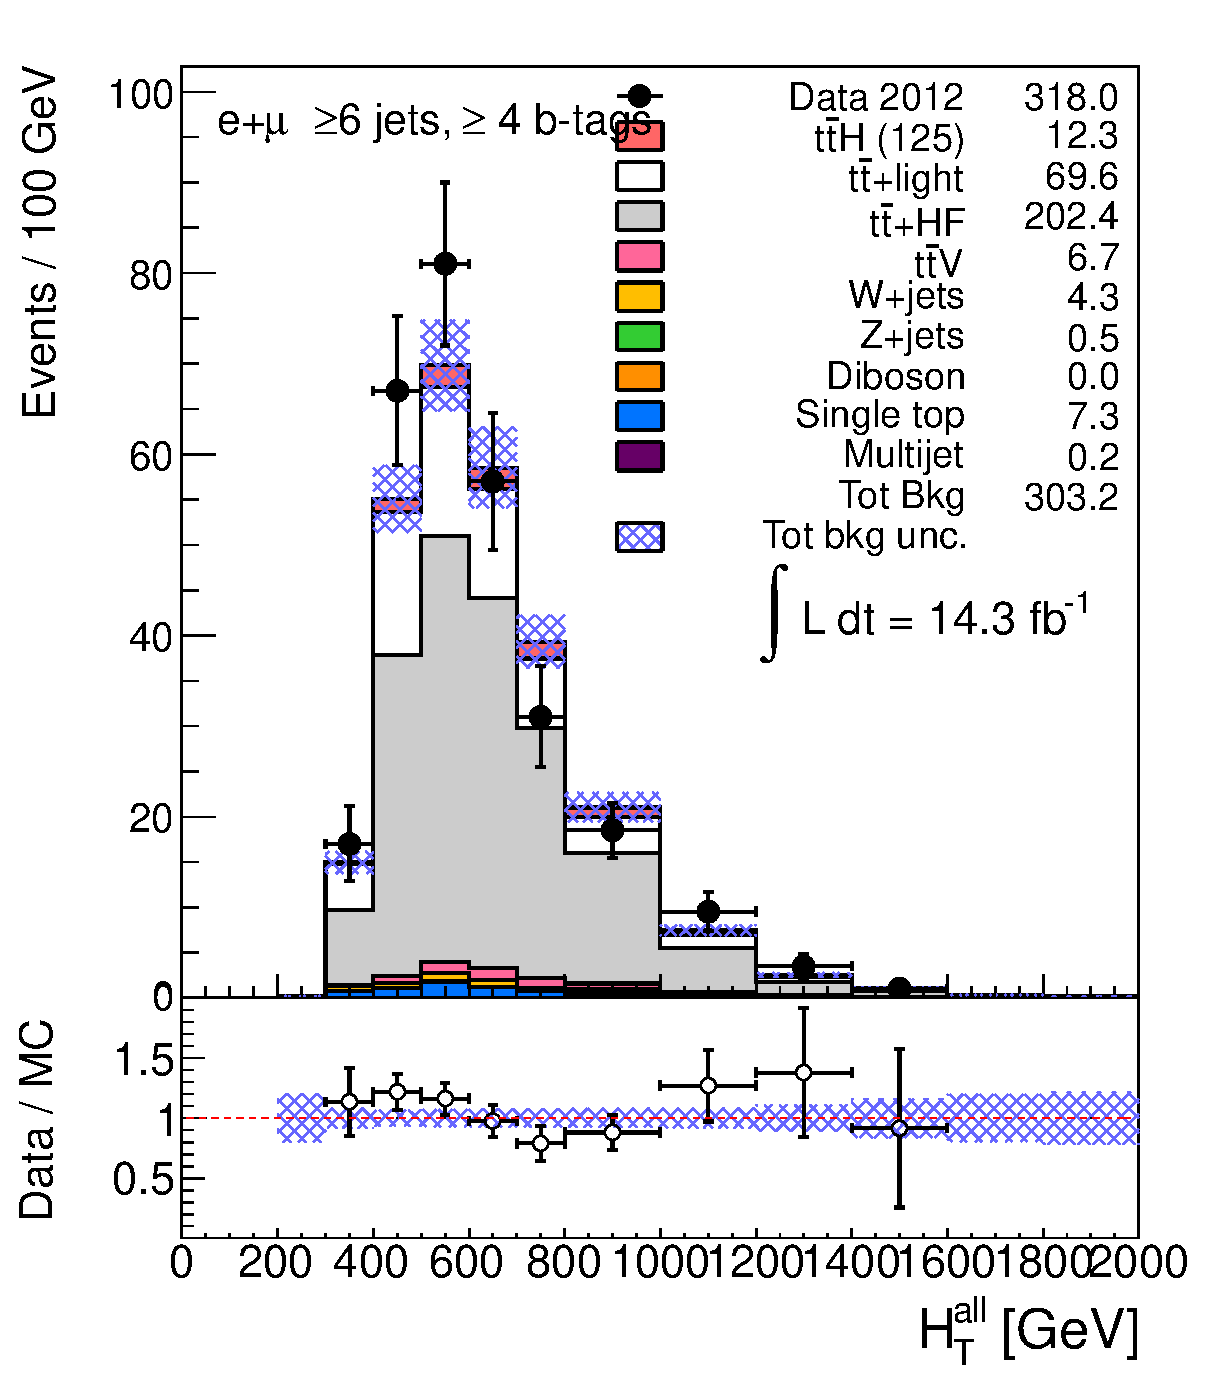
\includegraphics[width=.5\textwidth]{pics/combo/HTAll_6jetin4btagin_ELEMUON}
\includegraphics[width=.5\textwidth]{pics/combo/VLQAna_WbX_1W_MWb_4_ELEMUON_cutflow1234567_NOMINAL}

\end{minipage}\begin{minipage}{.5\textwidth}\centering
\myskip

The search channels do {\cccolor not overlap}\\
$\Downarrow$\\
can be combined in the statistical analysis\\
(consistent {\cccolor syst unc} treatment)


\begin{pgfpicture}{0.0\textwidth}{0.0\textheight}{1.\textwidth}{.9\textwidth}
   \begin{pgftranslate}{\pgfpoint{0.05\textwidth}{-0.02\textheight}}
\pgfdeclareimage[interpolate=true,width=.9\textwidth]{singlethtx}{pics/lim_singlet.pdf}
\pgfdeclareimage[interpolate=true,width=.9\textwidth]{singletcomb}{pics/combo/lim_singlet_comb.pdf}
%\pgfputat{\pgfxy(0.0,0.0)}{\pgfbox[left,base]{\pgfuseimage{mindr}}}
 \pgfsetlinewidth{1.pt}
 \usebeamercolor[bg]{head/foot boxes}
\pgfputat{\pgfxy(0.0,0.0)}{\pgfbox[left,base]{\pgfuseimage{singlethtx}}}
\pgfline{\pgfxy(3.35,0.1)}{\pgfxy(3.35,5.1)}
\pgfstroke
\only<1>{
 \pgfputat{\pgfxy(0.6,5.2)}{\pgfbox[left,base]{\cccolor \htx\ only: 640 (615)~\gev}}
}
\onslide<2->{
\pgfputat{\pgfxy(0.0,0.0)}{\pgfbox[left,base]{\pgfuseimage{singletcomb}}}
\pgfline{\pgfxy(3.5,0.1)}{\pgfxy(3.5,5.1)}
\pgfstroke
 \pgfputat{\pgfxy(1,5.2)}{\pgfbox[left,base]{\cccolor combination: 670 (675)~\gev}}
}
   \end{pgftranslate}

\end{pgfpicture}

\end{minipage}

\end{frame}



%%%%%%%%%%%%%%%%%%%%%%%%%
%%%
%%%%%%%%%%%%%%%%%%%%%%%%%
\begin{frame}\frametitle{Combined results}
\centering\footnotesize

\begin{minipage}{.35\textwidth}\centering

Individual analyses probe different areas

\begin{itemize}[<+->]
\item \wbx\ analysis alone very optimized for the bottom right corner
\item \htx\ gives general good coverage, brings complete exclusion up to {\cccolor 450~\gev\ } and almost excludes 650~\gev\ singlets
\item full combination reaches complete exclusion up to almost {\cccolor 600~\gev\ } and excludes 650~\gev\ singlets
\end{itemize}

\onslide<4->{
\dots but there's more from {\cccolor ATLAS Exotics}!
}

\end{minipage}\begin{minipage}{.65\textwidth}\centering

\begin{pgfpicture}{0.0\textwidth}{0.0\textheight}{1.\textwidth}{.6\textwidth}
   \begin{pgftranslate}{\pgfpoint{0.0\textwidth}{-0.15\textheight}}
\pgfdeclareimage[interpolate=true,width=1.\textwidth]{wbx}{pics/lim_Scan2D_tight_Bin1.pdf}
\pgfdeclareimage[interpolate=true,width=1.\textwidth]{htx}{pics/combo/htxT.png}
\pgfdeclareimage[interpolate=true,width=1.\textwidth]{comb}{pics/combo/combT.png}
\pgfdeclareimage[interpolate=true,width=1.\textwidth]{br2d}{pics/combo/lim_Scan2D_comb.pdf}
%\pgfputat{\pgfxy(0.0,0.0)}{\pgfbox[left,base]{\pgfuseimage{mindr}}}
 \pgfsetlinewidth{1.pt}
 \usebeamercolor[bg]{head/foot boxes}
\pgfputat{\pgfxy(0.0,0.0)}{\pgfbox[left,base]{\pgfuseimage{wbx}}}
\onslide<2->{
\pgfputat{\pgfxy(0.0,0.0)}{\pgfbox[left,base]{\pgfuseimage{htx}}}
}
\onslide<3->{
\pgfputat{\pgfxy(0.0,0.0)}{\pgfbox[left,base]{\pgfuseimage{comb}}}
}
\onslide<4->{
\pgfputat{\pgfxy(0.0,0.0)}{\pgfbox[left,base]{\pgfuseimage{br2d}}}
}
   \end{pgftranslate}

\end{pgfpicture}

\end{minipage}


\end{frame}

\FullBackgroundPicture{pics/ATLAS_VLQ_TT_june2013_step4}
%%%%%%%%%%%%%%%%%%%%%%%%%
%%%
%%%%%%%%%%%%%%%%%%%%%%%%%
\begin{frame}\frametitle{ATLAS BR plane coverage}%``worst case scenario'' coverage}
\centering\footnotesize

%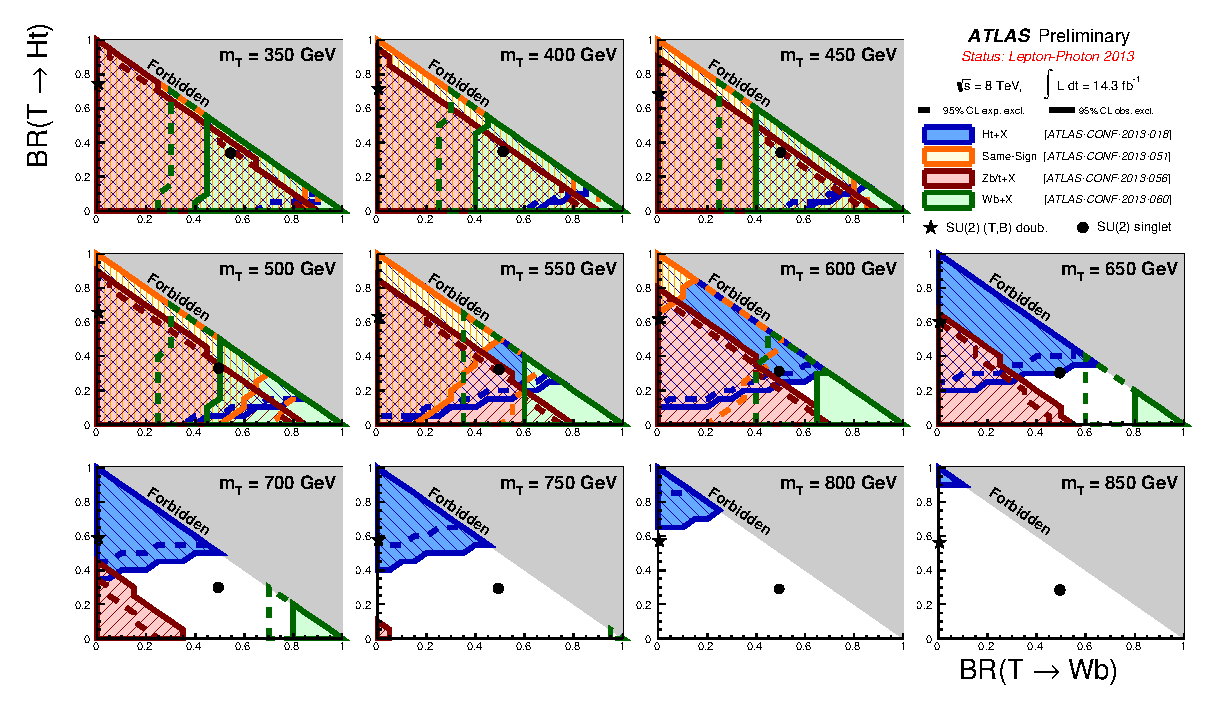
\includegraphics[width=0.8\textwidth]{pics/ATLAS_VLQ_TT_june2013_step4}

\end{frame}


\FullBackgroundPicture{pics/emptyIMG}
%%%%%%%%%%%%%%%%%%%%%%%%%
%%%
%%%%%%%%%%%%%%%%%%%%%%%%%
\begin{frame}\frametitle{Comparison to CMS results}
\centering\footnotesize

Inclusive \TTbar\ searches {\cccolor CMS-PAS-B2G-12-015~\cite{CMS-PAS-B2G-12-015}}
\myskip

\includegraphics[width=.34\textwidth]{pics/cms/triangle}
\includegraphics[width=.34\textwidth]{pics/cms/exptr}

\begin{tabular}{lclc}\toprule
\multicolumn{2}{c}{ATLAS single lepton} & \multicolumn{2}{c}{CMS single- and multi-lepton}\\\midrule
\multirow{2}{*}{Benchmark} & obs (exp) & \multirow{2}{*}{BR($Wb,Ht,Zt$)}  & obs (exp) \\
          & 95\% CL [GeV] & & 95\% CL [GeV] \\
Chiral & 740 (770) & (1.,0.,0.) & 700 (785)\\
Singlet & 670 (675) & (0.4,0.4,0.2) & 693 (766)\\
Doublet & 790 (745) & (0.,0.6,0.4) & 731 (783) \\
\bottomrule\end{tabular}


\end{frame}



